\documentclass[11pt]{article}
\usepackage{amssymb}
\usepackage{amsthm}
\usepackage{enumitem}
\usepackage{physics,amsmath}
\usepackage{bm}
\usepackage{adjustbox}
\usepackage{mathrsfs}
\usepackage{graphicx}
\usepackage{siunitx}
\usepackage[mathscr]{euscript}

\title{\textbf{Solved selected problems of Classical Mechanics - Gregory}}
\author{Franco Zacco}
\date{}

\addtolength{\topmargin}{-3cm}
\addtolength{\textheight}{3cm}

\newcommand{\hatr}{\bm{\hat{r}}}
\newcommand{\hatx}{\bm{\hat{x}}}
\newcommand{\haty}{\bm{\hat{y}}}
\newcommand{\hatz}{\bm{\hat{z}}}
\newcommand{\hatth}{\bm{\hat{\theta}}}
\newcommand{\hatphi}{\bm{\hat{\phi}}}
\newcommand{\hatrho}{\bm{\hat{\rho}}}
\theoremstyle{definition}
\newtheorem*{solution*}{Solution}

\begin{document}
\maketitle
\thispagestyle{empty}

\section*{Chapter 7 - Orbits in a central field}

	\begin{proof}{\textbf{7.1}}
        From the repulsive inverse cube field that we have
        $$\vectorbold{F} = \frac{m\gamma}{r^3} \hatr$$
        We can get the potential energy by solving the following ODE
        \begin{align*}
            \frac{\gamma}{r^3} &= -\frac{dV}{dr}\\
            \int dV &= -\gamma \int \frac{dr}{r^3}\\
            V &= \frac{\gamma}{2r^2}
        \end{align*}
        Also, we know that the apsidal distances equation is given by (assuming
        $\dot{r} = 0$)
        $$V(r) + \frac{L^2}{2r^2} = E$$
        Using the initial condition we know that $L = pv$ and $E = v^2/2$ (we are using
        $v$ instead of $V$ for the velocity to avoid confusion with the potential energy)
        then by replacing the values we have that the apsidal distances equation becomes
        \begin{align*}
            \frac{\gamma}{2r^2} + \frac{p^2v^2}{2r^2} &= \frac{v^2}{2}
        \end{align*} 
        So the distance of closest approach of $P$ is the positive root of  this
        equation then we have that 
        \begin{align*}
            \frac{1}{r^2}(\gamma + p^2v^2) &= v^2\\
            r &= \sqrt{\frac{\gamma}{v^2} + p^2}
        \end{align*}
    \end{proof}
	\begin{proof}{\textbf{7.3}}
        From the attractive inverse square field that we have
        $$\vectorbold{F} = -\frac{m\gamma}{r^2} \hatr$$
        We can get the potential energy by solving the following ODE
        \begin{align*}
            -\frac{dV}{dr} &= -\frac{\gamma}{r^2}\\
            \int dV &= \gamma \int \frac{dr}{r^2}\\
            V &= -\frac{\gamma}{r}
        \end{align*}
        Also, we know that the apsidal distances equation is given by (assuming
        $\dot{r} = 0$)
        $$V(r) + \frac{L^2}{2r^2} = E$$
        Then by replacing the value for $V$ and multiplying by $2r^2$ the entire
        equation we have that
        \begin{align*}
            -\frac{\gamma}{r} + \frac{L^2}{2r^2} &= E\\
            E + \frac{\gamma}{r} - \frac{L^2}{2r^2} &= 0 \\
            2Er^2 + 2\gamma r - L^2 &= 0
        \end{align*}
        So the solutions to this equation are
        \begin{align*}
            r &= \frac{-2\gamma \pm \sqrt{2^2\gamma^2 - 4 \cdot 2EL^2}}{2\cdot 2E}\\
              &= \frac{-\gamma \pm \sqrt{\gamma^2 - 2EL^2}}{2E}
        \end{align*}
        then by multiplying them we have that
        \begin{align*}
            r_1 \cdot r_2 &= 
            (-\frac{\gamma}{2E} + \frac{\sqrt{\gamma^2 - 2EL^2}}{2E})(-\frac{\gamma}{2E} -  \frac{\sqrt{\gamma^2 - 2EL^2}}{2E})\\
                &= \frac{\gamma^2}{4E^2} + \frac{\gamma\sqrt{\gamma^2 - 2EL^2}}{4E^2} - \frac{\gamma\sqrt{\gamma^2 - 2EL^2}}{4E^2} - \frac{\gamma^2 - 2EL^2}{4E^2}\\
                &= \frac{\gamma^2}{4E^2} - \frac{\gamma^2}{4E^2} - \frac{2EL^2}{4E^2}\\
                &= - \frac{L^2}{2E}
        \end{align*}
        And by summing them we get that 
        \begin{align*}
            r_1 + r_2 &= 
            (-\frac{\gamma}{2E} + \frac{\sqrt{\gamma^2 - 2EL^2}}{2E}) + (-\frac{\gamma}{2E} -  \frac{\sqrt{\gamma^2 - 2EL^2}}{2E})\\
                &= - \frac{\gamma}{E}
        \end{align*}
        On the other hand, we know that the orbit is an ellipse with $O$ as a focus then
        we know that
        \begin{align*}
            r_1 &= a - c = a(1 - c/a) = a(1 - e)\\
            r_2 &= a + c = a(1 + c/a) = a(1 + e)
        \end{align*}
        where $a$ is the semi-major axis, $c$ is the linear eccentricity and $e$ is the
        eccentricity.
        Again, by multiplying and summing these equations we get that
        \begin{align*}
            r_1 \cdot r_2 &= a(1 - e) \cdot a(1 + e)\\
                &= a^2(1 - e^2) = a^2(1 - 1 + \frac{b^2}{a^2}) = b^2\\\\
            r_1 + r_2 &= a(1 - e) + a(1 + e)\\
                &= 2a
        \end{align*}
        Finally, by joining the results we have that
        \begin{align*}
            -\frac{\gamma}{E} &= 2a\\
            E &= -\frac{\gamma}{2a}\\
        \end{align*}
        And for $L$
        \begin{align*}
            - \frac{L^2}{2E} &= b^2\\
            L^2 &= -2Eb^2\\
            L^2 &= -\frac{\gamma b^2}{a}
        \end{align*}

    \end{proof}
\cleardoublepage
	\begin{proof}{\textbf{7.6}}
        The force the comet experience because of the gravitational attractive inverse
        square field of the sun is given by
        $$\vectorbold{F} = - \frac{mMG}{r^2} \hatr$$
        Where $M$ is the mass of the sun and $G$ is the gravitational constant.
        Then
        $$f(1/u) = -MGu^2$$
        Also the angular momentum at the beginning is given by $L = pV$ where $p$ is
        the perpendicular distance to the sun and $V$ the initial velocity. So the
        path equation is given by
        $$\frac{d^2u}{d\theta^2} + u = -\frac{-MGu^2}{L^2u^2} = \frac{MG}{p^2V^2}$$
        And the solution to this equation is
        $$u = A\sin(\theta) + B\cos(\theta) + \frac{MG}{p^2V^2}$$
        Where we find the values of the constants $A$ and $B$ by using the initial
        conditions. When $r = \infty$ we have that $\theta = 0$ and therefore $u =0$
        which give us by plugging this values in the equation that $B = -MG / p^2V^2$.
        Also we know that
        $$\frac{du}{d\theta} = -\frac{\dot{r}}{L} = -\frac{-V}{pV} = \frac{1}{p}$$
        Then from the solution to the path equation we also have that
        \begin{align*}
            \frac{du}{d\theta} &= A\cos(\theta) - B\sin(\theta)
        \end{align*}
        so when $\theta=0$ we have that $A = 1/p$. Finally the solution to the path
        equation looks like
        $$u = \frac{1}{p}\sin(\theta) + \frac{MG}{p^2V^2}(1 - \cos(\theta))$$
        that is
        $$r = \frac{p}{\sin(\theta) + \frac{MG}{pV^2}(1 - \cos(\theta))}$$
        The comet goes to infinity when
        \begin{align*}
            \sin(\theta) + \frac{MG}{pV^2}(1 - \cos(\theta)) &= 0\\
            \frac{\sin(\theta)}{1-\cos(\theta)} &= -\frac{MG}{pV^2}\\
            \tan(\theta/2) &= -\frac{pV^2}{MG}\\    
        \end{align*}
        And the deflection angle happens for $\alpha = \pi - \theta$ then
        \begin{align*}
            \tan(\alpha/2) = \tan(\pi/2 - \theta/2) =
            \frac{\sin \pi/2 - \cos \theta/2}{\cos \pi/2 + \sin \theta/2} =
            \frac{1 - \cos \theta/2}{\sin \theta/2} = \tan(\theta/2)    
        \end{align*}        
        Therefore the deflection angle is
        $$\alpha = 2\tan^{-1}\left(-\frac{pV^2}{MG}\right)$$
        The minimum value of $r$ we can get (i.e the closest approach) is going to
        happen when $\sin(\theta) + x(1 - \cos(\theta))$ is maximum where
        $x = \frac{MG}{pV^2}$ and $0\leq\theta\leq \pi + \alpha$.
    \end{proof}
	\begin{proof}{\textbf{7.8}}
        The force the particle experience because of the central field where it is in
        is given by
        $$\vectorbold{F} = - \frac{m\gamma^2}{r^5} \hatr$$
        Then
        $$f(1/u) = -\gamma^2u^5$$
        Also the angular momentum at the beginning is given by
        $L = p\sqrt{2}\gamma /p^2 = \sqrt{2}\gamma / p$
        where $p$ is the perpendicular distance to $O$.
        So the path equation is given by
        $$\frac{d^2u}{d\theta^2} + u = -\frac{(-\gamma^2u^5)}{(\sqrt{2}\gamma / p)^2u^2} =
        \frac{p^2u^3}{2}$$
        If we define $v = du/d\theta$ then
        $$\frac{d^2u}{d\theta^2} = \frac{dv}{d\theta} = \frac{dv}{du}\frac{du}{d\theta}
        = \frac{dv}{du}v$$
        and this means that
        \begin{align*}
            \frac{dv}{du}v &= \frac{p^2u^3}{2} - u\\
            \int v dv &= \frac{p^2}{2}\int u^3 du - \int u du\\
            \frac{v^2}{2} &= \frac{p^2}{2} \frac{u^4}{4} - \frac{u^2}{2} +C\\
            \left(\frac{du}{d\theta}\right)^2 &= p^2\frac{u^4}{4} - u^2 + 2C
        \end{align*}
        And by using the initial conditions if $r = \infty$ then $u = 0$ and $\theta = 0$
        also $du/d\theta = -\dot{r}/L = 1/p$ so $C = 1/2p^2$.\\
        Finally, this equation is a separable ODE so we have that 
        \begin{align*}
            \left(\frac{du}{d\theta}\right)^2 &= p^2\frac{u^4}{4} - u^2 + \frac{1}{p^2}\\
            \frac{du}{d\theta} &= \sqrt{\frac{1}{4p^2} (u^4p^4 - 4p^2u^2 + 4)}\\
            \frac{du}{d\theta} &=\frac{1}{2p} \sqrt{(u^2p^2 - 2)^2}\\
            \frac{du}{d\theta} &=\frac{1}{2p} (u^2p^2 - 2)\\
            \theta &= 2p \int \frac{du}{u^2p^2 - 2}\\
            \theta &= \frac{2}{p} \int \frac{du}{u^2 - 2/p^2}\\
            \theta &= -\sqrt{2}\tanh^{-1}(up/\sqrt{2})\\
            \tanh(-\frac{\theta}{\sqrt{2}}) &= \frac{up}{\sqrt{2}}\\
            r &= \frac{p}{\sqrt{2}}\coth(\frac{\theta}{\sqrt{2}})
        \end{align*}
        Where we used that $1/\tanh(x) = \coth(x)$ and that $\tanh(-x) = -\tanh(x)$ and
        we eliminate the minus sign by taking $-\sqrt{2}$. 
    \end{proof}
	\begin{proof}{\textbf{7.11}}
        Since the planet experiences a force field of the form
        $$\vectorbold{F} = - \frac{m\gamma}{r^2}(1 + \frac{\epsilon a^2}{r^2}) \hatr$$
        Then we have that
        $$f(r) = - \frac{\gamma}{r^2}(1 + \frac{\epsilon a^2}{r^2})$$
        and the derivative of this expression is given by
        $$f'(r) = \frac{2\gamma}{r^3} + \frac{4\gamma\epsilon a^2}{r^5}$$
        On the other hand, the coefficient of $\xi$ in the path equation in terms of the
        perturbation we know it is
        $$\Omega^2 \equiv 3 + \frac{af'(a)}{f(a)}$$
        Then in this case we have that
        \begin{align*}
            \Omega^2 &= 3 + \frac{a(\frac{2\gamma}{a^3} + \frac{4\gamma\epsilon a^2}{a^5})}
            {- \frac{\gamma}{a^2}(1 + \frac{\epsilon a^2}{a^2})} \\
            \Omega^2 &= 3 - \frac{(\frac{2\gamma}{a^2} + \frac{4\gamma\epsilon}{a^2})}
            {\frac{\gamma}{a^2}(1 + \epsilon)}
             =3 - \frac{2(1 + 2\epsilon)}{(1 + \epsilon)}\\
            \Omega^2 &= \frac{3+3\epsilon - (2 + 4\epsilon)}{(1 + \epsilon)}
            = \frac{1-\epsilon}{1 + \epsilon}
            % \Omega^2 &= \frac{(1 -4\epsilon)(1+\epsilon)}{(1 + \epsilon)} = (1 -4\epsilon)
        \end{align*}
        Finally since we know that $\epsilon$ is small we can approximate it by its
        binomial approximation
        \begin{align*}
            \Omega &= \frac{(1-\epsilon)^{1/2}}{(1+\epsilon)^{1/2}}
            = \frac{1-\epsilon/2 + O(\epsilon^2)}{1+\epsilon/2 + O(\epsilon^2)}
        \end{align*}
        Then the apsidal angle is given by
        $$ \alpha = \frac{\pi}{\Omega} = \frac{\pi(1+\epsilon/2 + O(\epsilon^2))}{1-\epsilon/2 + O(\epsilon^2)} = 
        \pi(1 + \epsilon) + O(\epsilon^2)$$
        Therefore the perihelion will advance annually by $2\pi\epsilon$.
    \end{proof}
	\begin{proof}{\textbf{7.12}}
        Due to the dust cloud of uniform density the planet experiences a force field
        given by
        $$\left(\frac{4}{3}\pi r^3 \frac{\epsilon M}{a^3}\right) \frac{mG}{r^2} =
        \frac{4}{3}\frac{mMG\epsilon\pi r}{a^3}$$
        Where $\left(\frac{4}{3}\pi r^3 \frac{\epsilon M}{a^3}\right)$ is the volume of
        a sphere of radius $r$ times the density of the dust cloud. Then the total
        inward force the planet experience is
        $$\vectorbold{F} = \frac{mMG}{r^2} + \frac{4}{3}\frac{mMG\epsilon\pi r}{a^3} \hatr$$
        So if we assume that the planet is in a nearly circular orbit then we calculate
        $$f(r) = \frac{\gamma}{r^2} + \frac{4}{3}\frac{\gamma\epsilon\pi r}{a^3}$$
        and
        $$f'(r) = -\frac{2\gamma}{r^3} + \frac{4}{3}\frac{\gamma\epsilon\pi }{a^3}$$
        Where in this case $\gamma = MG$. Now we can calculate $\Omega$ as follows
        \begin{align*}
            \Omega^2 &= 3 + \frac{af'(a)}{f(a)}
                = 3 + \frac{-\frac{2\gamma}{a^2} + \frac{4}{3}\frac{\gamma\epsilon\pi }{a^2}}
                {\frac{\gamma}{a^2} + \frac{4}{3}\frac{\gamma\epsilon\pi }{a^2}}\\
                &= 3 + \frac{\gamma(-2 + \frac{4}{3} \epsilon \pi)}
                {\gamma(1 + \frac{4}{3}\epsilon \pi)}
                = \frac{3 + 4\pi\epsilon -2 + \frac{4}{3}\pi\epsilon}{1 + \frac{4}{3}\pi\epsilon}\\
                &= \frac{1 + \frac{16}{3} \epsilon \pi}{1 + \frac{4}{3}\epsilon \pi}
        \end{align*}
        Finally since we know that $\epsilon$ is small we can approximate it by its
        binomial approximation
        \begin{align*}
            \Omega &= \frac{(1 + \frac{16}{3} \epsilon \pi)^{1/2}}
            {(1 + \frac{4}{3}\epsilon \pi)^{1/2}}
            = \frac{1+\frac{8}{3}\epsilon\pi + O(\epsilon^2)}
            {1+\frac{2}{3}\epsilon\pi + O(\epsilon^2)}
        \end{align*}
        Then the apsidal angle is given by
        $$\alpha = \frac{\pi}{\Omega} = \frac{\pi(1+\frac{2}{3}\epsilon\pi + O(\epsilon^2))}
        {1+\frac{8}{3}\epsilon\pi + O(\epsilon^2)} = \pi(1 - 2\pi\epsilon) + O(\epsilon^2)$$
        Therefore the perihelion will advance annually by $-4\pi^2\epsilon$.
    \end{proof}
\cleardoublepage
	\begin{proof}{\textbf{7.13}}
        We know that the planet's gravitational force field according to general
        relativity is
        $$\frac{d^2u}{d\theta^2} + u = \frac{MG}{L^2} + \left(\frac{3MG}{c^2}\right)u^2$$
        Then we can write that
        \begin{align*}
            \frac{f(1/u)}{L^2u^2} &= \frac{MG}{L^2} + \left(\frac{3MG}{c^2}\right)u^2\\
            f(1/u) &= MGu^2 + \left(\frac{3MGL^2}{c^2}\right)u^4
        \end{align*}
        So, since we know $c$ is big then we can define $\epsilon = L^2/c^2a^2$ and
        if we name $\gamma = MG$ we get that
        $$f(r) = \frac{\gamma}{r^2} + \frac{3\gamma\epsilon a^2}{r^4}$$
        Then $f'(r)$ is given by
        $$f'(r) = -\frac{2\gamma}{r^3} - \frac{12\gamma\epsilon a^2}{r^5}$$
        Now let us calculate $\Omega$ as follows
        \begin{align*}
            \Omega^2 &= 3 + \frac{af'(a)}{f(a)}
                = 3 + \frac{-(\frac{2\gamma}{a^2} + \frac{12\gamma\epsilon}{a^2})}
                {\frac{\gamma}{a^2} + \frac{3\gamma\epsilon}{a^2}}\\
                &= 3 - \frac{2\gamma + 12\gamma\epsilon}{\gamma + 3\gamma\epsilon}
                = \frac{1 - 3\epsilon}{1 + 3\epsilon}
        \end{align*}
        Finally since we know that $\epsilon$ is small we can approximate it by its
        binomial approximation
        \begin{align*}
            \Omega &= \frac{(1 - 3\epsilon)^{1/2}}
            {(1 + 3\epsilon)^{1/2}}
            = \frac{1 - \frac{3}{2}\epsilon + O(\epsilon^2)}
            {1 + \frac{3}{2}\epsilon + O(\epsilon^2)}
        \end{align*}
        Then the apsidal angle is given by
        $$\alpha = \frac{\pi}{\Omega}
        = \frac{\pi(1+\frac{3}{2}\epsilon + O(\epsilon^2))}
        {1-\frac{3}{2}\epsilon + O(\epsilon^2)}
        = \pi(1 + 3\epsilon) + O(\epsilon^2)$$
        Therefore the perihelion will advance annually by $6\pi\epsilon$.
    \end{proof}
\cleardoublepage
	\begin{proof}{\textbf{7.14}}
        In this case we are in the situation shown below
        \begin{center}
            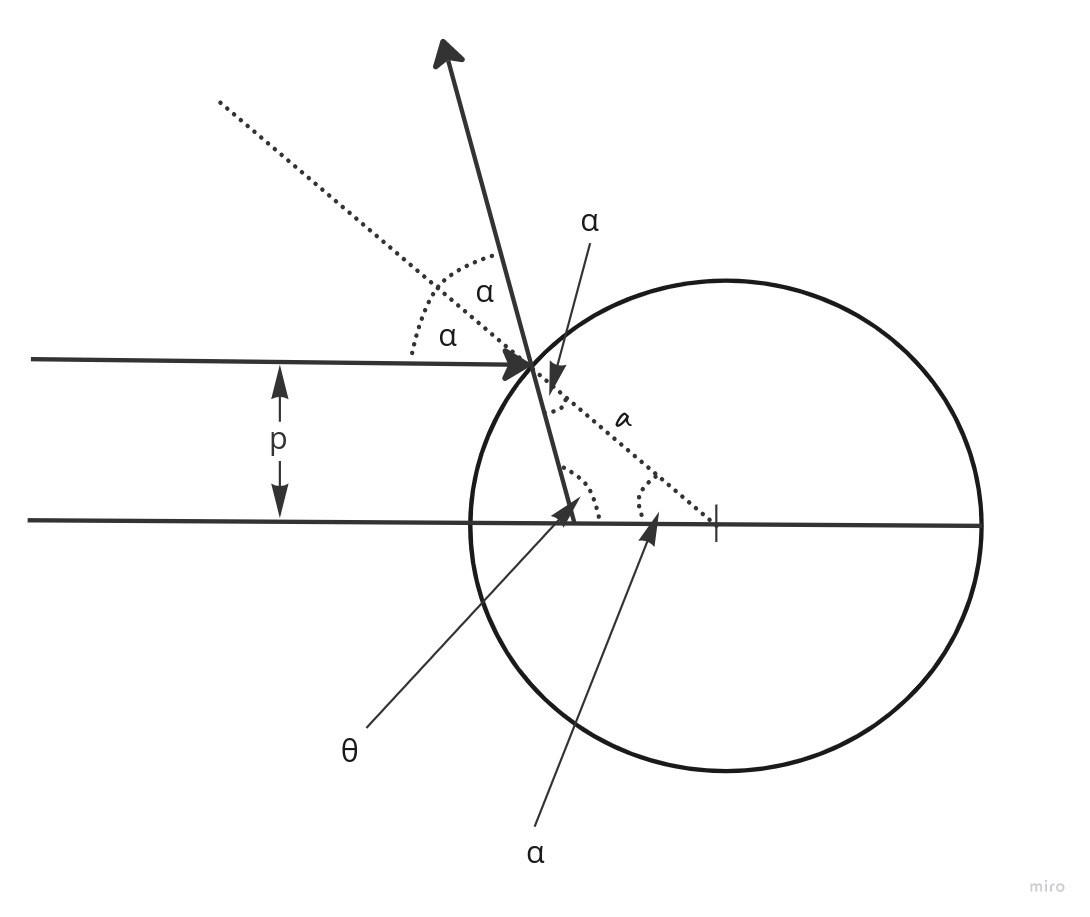
\includegraphics[scale=0.2]{ch7-14.jpg}
        \end{center}
        Where $p$ is the impact parameter and $\theta$ is the reflected angle, then we
        have that
        $$p = a\sin(\alpha)$$ 
        Also $\theta = \pi - 2\alpha$ so from there we can write $p$ in terms of $\theta$
        as follows
        $$p = a\sin(\frac{\pi - \theta}{2}) = -a\cos(\frac{\theta}{2})$$
        Then since this is a axisymmetric scattering cross section we have that the
        differential scattering cross section is given by
        \begin{align*}
            \sigma(\theta) &= -\frac{p}{\sin(\theta)}\frac{dp}{d\theta}\\
                &= \frac{a\cos(\theta/2)}{\sin(\theta)}\frac{a\sin(\theta/2)}{2}
                = \frac{a^2}{2\sin(\theta)}\frac{\sin(\theta)}{2}\\
                &= \frac{a^2}{4}
        \end{align*}
        Finally, the total scattering cross section is
        \begin{align*}
            S &= \int_{0}^{\pi}\int_{0}^{2\pi}\sigma(\theta)\sin(\theta)d\theta d\phi\\
              &= \frac{a^2}{4}\int_{0}^{\pi}\sin(\theta)d\theta\int_{0}^{2\pi}d\phi\\
              &= \frac{a^2\pi}{2}\int_{0}^{\pi}\sin(\theta)d\theta\\
              &= \frac{a^2\pi}{2}\left[-\cos(\theta)\right]_{0}^{\pi}\\
              &= a^2\pi
        \end{align*}
    \end{proof}
	\begin{proof}{\textbf{7.19}}
        Just before the spacecraft fires the engines, from the Energy conservation
        expression we have that
        $$\frac{1}{2}V^2 = \frac{1}{2}v^2 - \frac{\gamma}{c}$$
        Where we are using that $E = \frac{1}{2}V^2$ when the spacecraft is far away,
        $\gamma = MG$ where $M$ is the mass of the planet and $v$ is the velocity
        just before the spacecraft fires the engines. Then $v$ is given by
        $$v = \sqrt{V^2 + \frac{2\gamma}{c}}$$
        The kinetic energy at the moment we fire the engines is going to be
        $$\frac{1}{2}(kv)^2 = \frac{1}{2}k^2(V^2 + \frac{2\gamma}{c})$$
        Therefore the total energy at the moment we fire the engines is going to be
        $$E = \frac{1}{2}k^2(V^2 + \frac{2\gamma}{c}) - \frac{\gamma}{c}$$
        And for the spacecraft to go into orbit we need that $E < 0$ so this means that
        we need that
        \begin{align*}
            \frac{1}{2}k^2(V^2 + \frac{2\gamma}{c}) &< \frac{\gamma}{c}\\
            k^2 &< \frac{2\gamma}{c}\frac{1}{V^2 + \frac{2\gamma}{c}}\\
            k &< \sqrt{\frac{2\gamma}{cV^2 + 2\gamma}}\\
        \end{align*}
    \end{proof}
\cleardoublepage
	\begin{proof}{\textbf{7.20}}
        We want to compute the following integral
        \begin{align*}
            \bar{V} &= \frac{1}{T}\int_0^T Vdt\\
                &= \frac{1}{T}\int_0^T -\frac{\gamma}{r}dt\\
                &= -\frac{\gamma}{T}\int_0^{2\pi} \frac{1}{r}\frac{dt}{d\theta}d\theta\\
                &= -\frac{\gamma}{T}\int_0^{2\pi} \frac{r}{r^2\dot{\theta}}d\theta\\
                &= -\frac{\gamma}{T}\int_0^{2\pi} \frac{r}{L}d\theta\\
        \end{align*}
        We also know that $r = \frac{b^2}{a(1+e\cos\theta)}$ so we have that
        \begin{align*}
            \bar{V} &= -\frac{\gamma b^2}{TLa}\int_0^{2\pi} \frac{1}{1 + e\cos\theta}d\theta\\
        \end{align*}
        Now we can change variables again from $\theta$ to $\psi$ knowing that
        $$\frac{d\theta}{d\psi} = \frac{b}{a(1-e\cos\psi)} \quad\text{and that}\quad
        (1-e\cos\psi)(1+e\cos\theta) = \frac{b^2}{a^2}$$
        Then
        \begin{align*}
            \bar{V} &= -\frac{\gamma b^2}{TLa}\int_0^{2\pi} \frac{1}{1 + e\cos\theta}
            \frac{d\theta}{d\psi} d\psi\\
                &= -\frac{\gamma b^3}{TLa^2}\int_0^{2\pi} \frac{1}{(1 + e\cos\theta)}
            \frac{1}{(1-e\cos\psi)} d\psi\\
                &= -\frac{\gamma b}{TL}\int_0^{2\pi}d\psi\\
                &= -2\pi\frac{\gamma b}{TL}\\
        \end{align*}
        Finally, using the equations we have for the period
        $T = 2\pi\sqrt{\frac{a^3}{\gamma}}$ and the angular momentum
        $L = \sqrt{\gamma \frac{b^2}{a}}$ we get that
        \begin{align*}
            \bar{V} &= -\frac{2\pi \gamma b}{2\pi \sqrt{\frac{a^3}{\gamma}}\sqrt{\gamma \frac{b^2}{a}}}
            = -\frac{\gamma}{a}
        \end{align*}
        Since we know the orbit is elliptical then the total energy is $E = -\gamma/2a$
        So we can calculate the time average of the kinetic energy as follows
        \begin{align*}
            \bar{T} + \bar{V} &= -\frac{\gamma}{a}\\
            \bar{T} &= -\frac{\gamma}{2a} + \frac{\gamma}{a}\\
            \bar{T} &= \frac{\gamma}{2a}
        \end{align*}
    \end{proof}
    \begin{proof}{\textbf{7.21}}
        We want to compute the following integral
        \begin{align*}
            \bar{r} &= \frac{1}{\tau}\int_0^\tau r~dt\\
                &= \frac{1}{\tau}\int_0^{2\pi} r\frac{dt}{d\theta}d\theta\\
                &= \frac{1}{\tau}\int_0^{2\pi} \frac{r^3}{r^2\dot{\theta}}d\theta\\
                &= \frac{1}{\tau L}\int_0^{2\pi} r^3 d\theta\\
        \end{align*}
        We also know that $r = \frac{b^2}{a(1+e\cos\theta)}$ so we have that
        \begin{align*}
            \bar{r} &= \frac{1}{\tau L}\int_0^{2\pi} \frac{b^6}{a^3(1+e\cos\theta)^3} d\theta\\
                &= \frac{b^6}{\tau La^3}\int_0^{2\pi} \frac{1}{(1+e\cos\theta)^3} d\theta
        \end{align*}
        Now we can change variables again from $\theta$ to $\psi$ knowing that
        $$\frac{d\theta}{d\psi} = \frac{b}{a(1-e\cos\psi)} \quad\text{and that}\quad
        (1-e\cos\psi)(1+e\cos\theta) = \frac{b^2}{a^2}$$
        Then
        \begin{align*}
            \bar{r} &= \frac{b^7}{\tau La^4}\int_0^{2\pi} \frac{1}{(1+e\cos\theta)^3(1-e\cos\psi)}
                 d\psi\\
                 &= \frac{b^5}{\tau La^2}\int_0^{2\pi} \frac{1}{(1+e\cos\theta)^2} d\psi\\
                 &= \frac{b^5}{\tau La^2}\int_0^{2\pi} \frac{(1-e\cos\psi)^2}{(1+e\cos\theta)^2(1-e\cos\psi)^2}
                 d\psi\\
                 &= \frac{a^2b}{\tau L}\int_0^{2\pi} (1-e\cos\psi)^2 d\psi
        \end{align*}
        Therefore solving the integral and using the equations we have for $\tau$ and $L$ 
        we have that
        \begin{align*}
            \bar{r} &= \frac{\pi a^2 b}{\tau L}(e^2+2)\\
                &= \frac{\pi a^2 b}{2\pi \sqrt{a^3/\gamma} \sqrt{\gamma b^2/a}}(e^2+2)\\
                &= \frac{a}{2}(e^2+2) = a (1+\frac{e^2}{2})
        \end{align*}

    \end{proof}
    \begin{proof}{\textbf{7.22}}
        Let us take the following plot of the Hohmann transfer we need to perform
        \begin{center}
            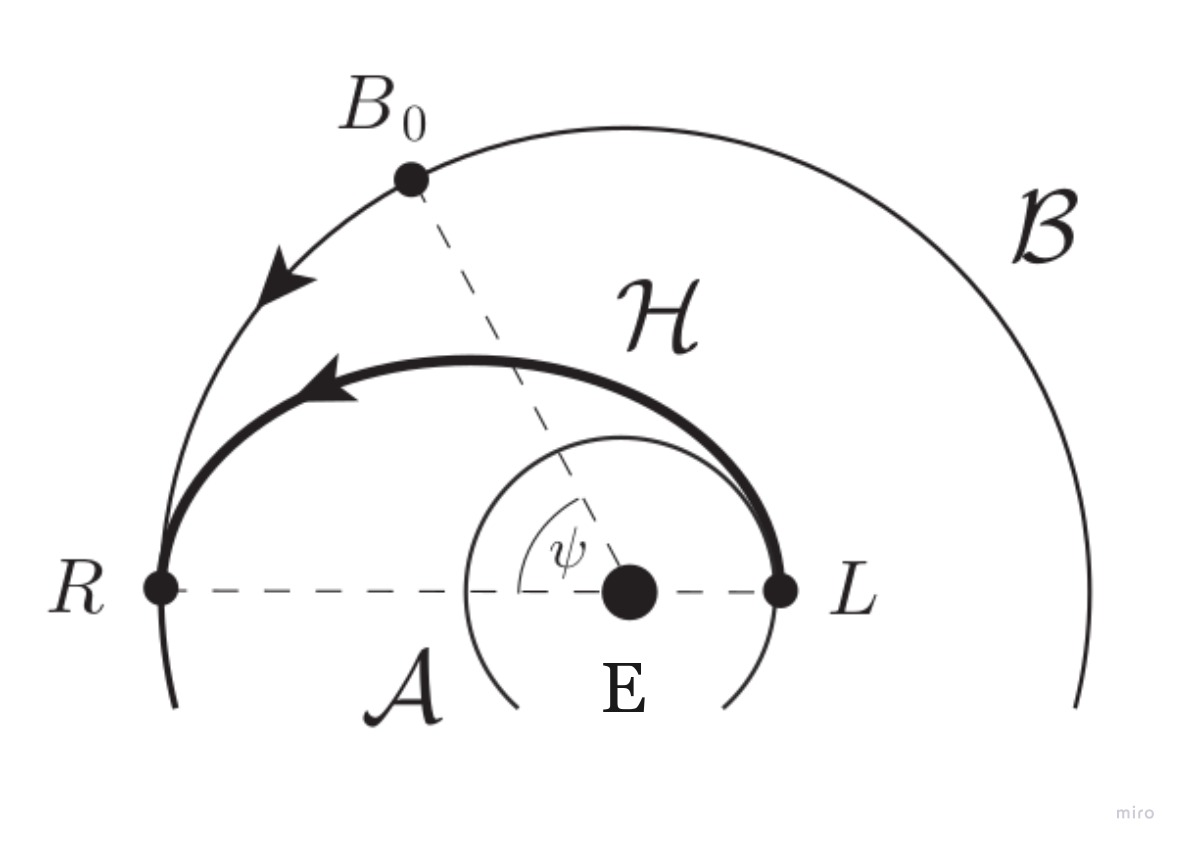
\includegraphics[scale=0.2]{./ch7-22.jpg}
        \end{center}
        Where $E$ is the Earth, $A$ and $B$ are the initial orbit and the
        end orbit we want to reach respectively. So given that we perform two firings of
        the motors there are two velocity changes and therefore we want to minimize $Q$
        where
        $$Q = |\Delta v^E| + |\Delta v^M|$$
        Since the perihelial and aphelial distances in the Hohmann orbit are $A$ and $B$
        it follows that
        $$A = a(1-e) \quad\quad B =a(1+e)$$
        so that the geometrical parameters of the orbit are given by
        $$a=\frac{1}{2}(B + A) \quad\quad e = \frac{B - A}{B + A}$$
        The angular momentum $L$ of the orbit is then given by the L-formula to be
        $$L^2 = \frac{\gamma b^2}{a} = \gamma(1-e^2)a = \frac{\gamma BA}{B+A}$$
        Where $\gamma = MG = R^2g = 398903.12~km^3/s^2$ and there $R$ is the radius of
        the Earth and $g$ is the gravity acceleration.\\
        From $L$ we can find the speed $V^L$ of the spacecraft just after the lift-off
        firing, and the speed $V^R$ at the rendezvous point just before the second firing.
        These are
        $$V^L = \sqrt{\frac{2\gamma B}{A(B+A)}} \quad\quad
        V^R = \sqrt{\frac{2\gamma A}{B(B+A)}}$$
        So
        $$\Delta v^E = V^L - v^E \quad\quad \Delta v^M = v^M - V^R$$
        Where $v^E$ is the velocity of the spacecraft in the orbit around the Earth
        before the firing and and $v^M$ is the velocity that the spacecraft should get 
        to orbit around the Moon. Then
        $$\Delta v^E = \sqrt{\frac{2\gamma B}{A(B+A)}} - \sqrt{\frac{\gamma}{A}}$$
        $$\Delta v^M = \sqrt{\frac{\gamma}{B}} - \sqrt{\frac{2\gamma A}{B(B+A)}}$$
        Then the travel time $T$, which is half the period of the Hohmann orbit, is
        given by
        $$T^2 = \frac{\pi^2 a^3}{\gamma} = \frac{\pi^2 (B+A)^3}{8 \gamma}$$
        Now we can plug in the values of $A = 6580~km$ and $B=384000~km$ to get
        $$\Delta v^E = 10.91 - 7.78 = 3.13~km/s$$
        $$\Delta v^M = 1.019-0.187 = 0.832~km/s$$
        And 
        $$T = 429275.56~s = 119.24~h$$
    \end{proof}
\cleardoublepage
    \begin{proof}{\textbf{7.23}}
        To find the most fuel efficient method of escaping from earth let us first
        compute the energy the spacecraft has at the moment of the engine firing
        \begin{align*}
            E &= \frac{1}{2}(\vectorbold{v} + \Delta\vectorbold{v})^2 - \frac{\gamma}{r}\\
              &= \frac{1}{2}\vectorbold{v}^2 + \vectorbold{v}\cdot \Delta\vectorbold{v} +
              \frac{1}{2}\Delta\vectorbold{v}^2 - \frac{\gamma}{r}\\
              &= \vectorbold{v}\cdot \Delta\vectorbold{v} +
              \frac{1}{2}\Delta\vectorbold{v}^2 + E' 
        \end{align*}
        Where $E'$ is the energy before firing the engine. So to exit the elliptical orbit
        we need that $E \geq 0$ then this means that
        $$\vectorbold{v}\cdot \Delta\vectorbold{v} + \frac{1}{2}\Delta\vectorbold{v}^2
        \geq -E'$$
        We know that the maximum value of the dot product happens when both vectors are
        parallel so $\Delta \vectorbold{v}$ must be parallel to $\vectorbold{v}$.
        Then what is left to decide is when is the right moment to fire the engine, and
        this would be when $\vectorbold{v}$ is maximum to minimize the value of
        $\Delta \vectorbold{v}$ we need. Since we know that the velocity of an object in
        an elliptical orbit is given by
        $$v = \sqrt{\gamma(\frac{2}{r} - \frac{1}{a})}$$
        We have that the highest velocity will happen when the object is closest to the
        focal point. Therefore the perigee of the orbit.
    \end{proof}
\cleardoublepage
    \begin{proof}{\textbf{7.26}}
        From the Newton equations of motion we have for the radial components the
        following
        \begin{align*}
            m(\ddot{r} - r\dot{\theta}^2) &= -\frac{m\gamma}{r^2} - mK\dot{r}\\
            \ddot{r} + K\dot{r} + \frac{\gamma}{r^2} - r\dot{\theta}^2  &= 0
        \end{align*}
        And for the angular component knowing that $\ddot{\theta} = 0$ we get that
        \begin{align*}
            m(r\ddot{\theta} + 2\dot{r}\dot{\theta}) &= - mKr\dot{\theta}\\
            2\dot{r} &= - Kr\\
            2 \int \frac{dr}{r} &= -K \int dt\\ 
            2 \log(r) &= -Kt + C\\
            r &=  e^{-Kt/2}e^{C}
        \end{align*}
        Since $\ddot{\theta} = 0$ then this means that $\dot{\theta}$ is a constant then
        we can write the following
        \begin{align*}
            r^2\dot{\theta} &= e^{-Kt}e^{2C}\dot{\theta} \\
            r^2\dot{\theta} &= L_0e^{-Kt}
        \end{align*}
        Where we defined $L_0 = e^{2C}\dot{\theta}$. Finally we can re write the first
        equation we derived as
        $$\ddot{r} + K\dot{r} + \frac{\gamma}{r^2} - \frac{L_0^2e^{-2Kt}}{r^3} = 0\\$$
        Let us now neglect the terms $\dot{r}$ and $\ddot{r}$ then we have that
        \begin{align*}
            \frac{\gamma}{r^2} &= \frac{L_0^2e^{-2Kt}}{r^3}\\
            r &= \frac{L_0^2e^{-2Kt}}{\gamma}
        \end{align*}
        Since $r$ is a function of $e^{-2Kt}$ which decreases slowly we see that the
        orbit slowly contracts.
        Replacing the value of $r$ in the formula for $r^2\dot{\theta}$ we get that
        \begin{align*}
            \dot{\theta} &= \frac{\gamma^2}{L_0^3e^{-3Kt}}
        \end{align*}
        Finally, we have that
        $$v = r \dot{\theta} = \frac{\gamma}{L_0e^{-Kt}}$$
        Therefore since $v$ is a function of $e^{Kt}$ we see that $v$ increases over
        time.
    \end{proof}

\end{document}






















